\documentclass{beamer}
\usepackage{presentation}

\begin{document}

\frame{\titlepage}

\begin{frame}
  \frametitle{Introduction}
  \begin{quote}{}
    Single Purpose Cloud Connected Tablet for organizing scheduled items by necessity, urgency and frequency
  \end{quote}

  \begin{minipage}{0.33\textwidth}
    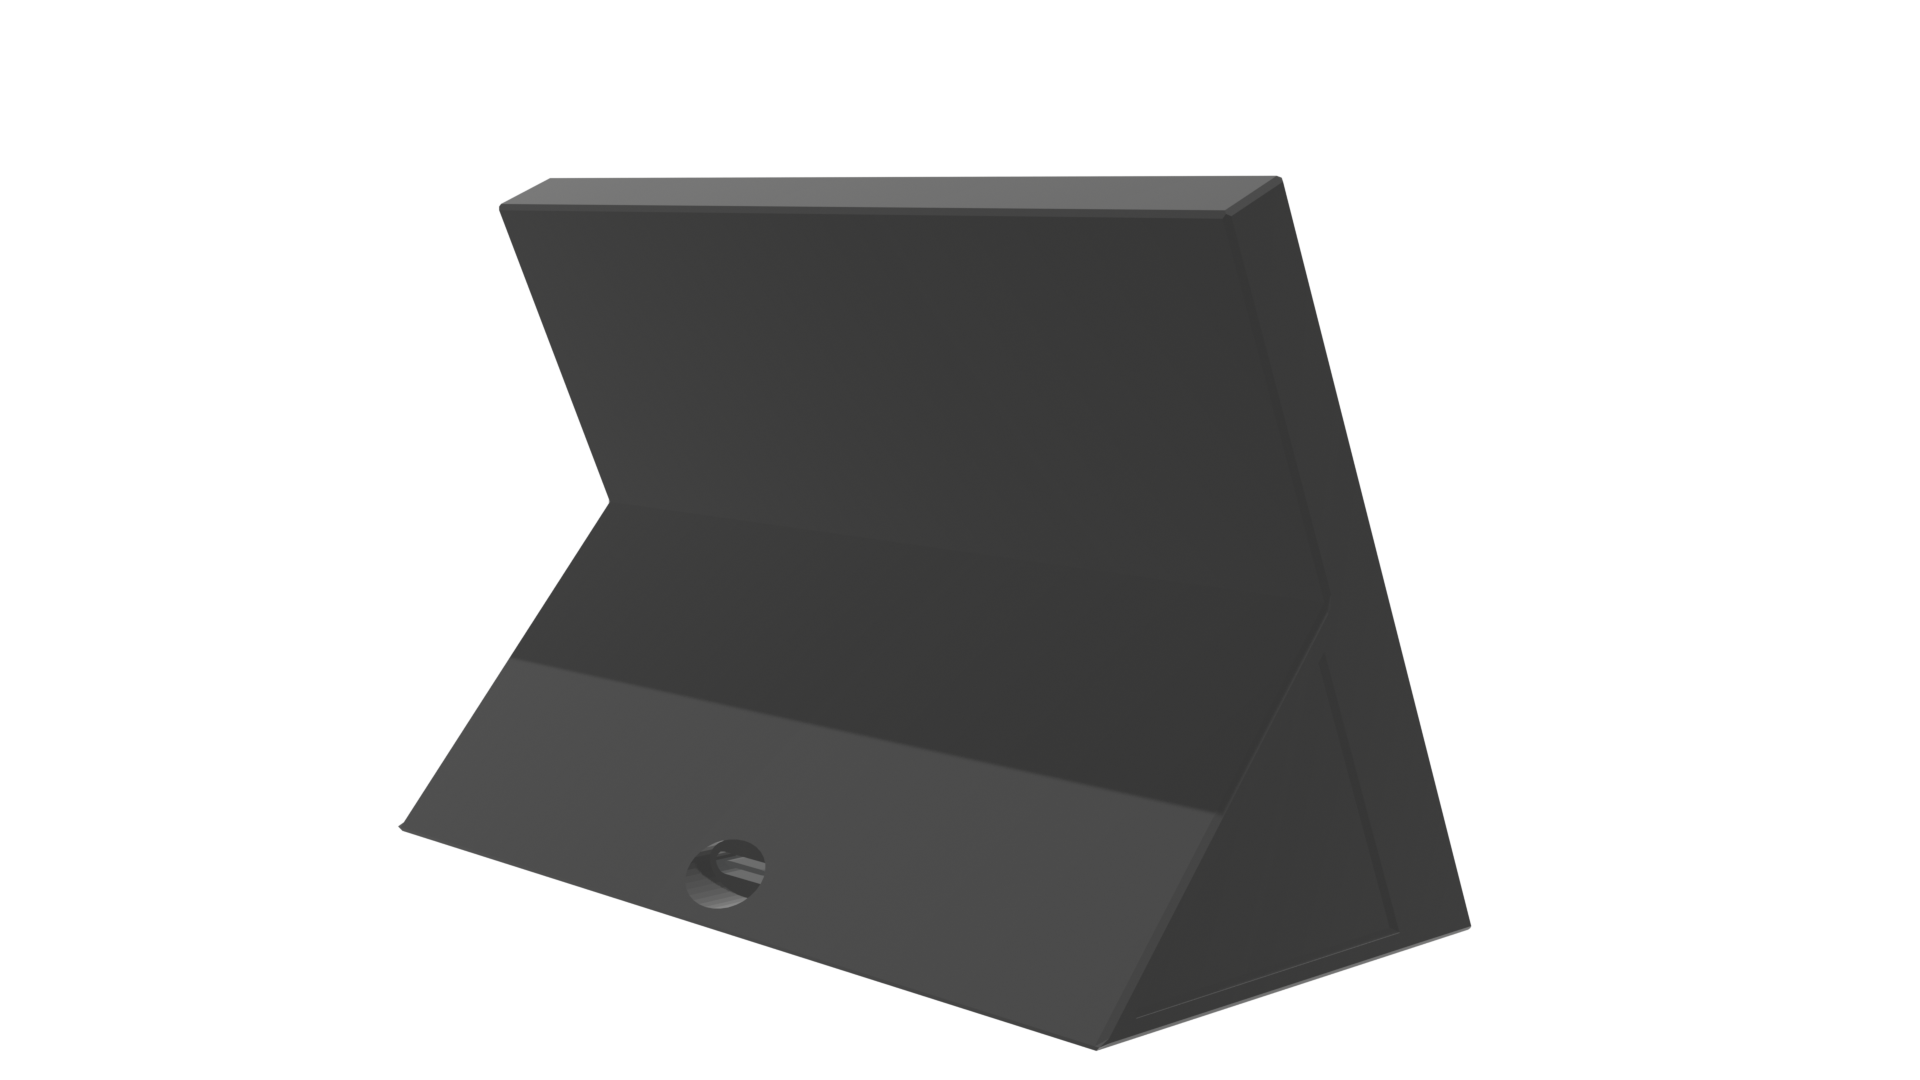
\includegraphics[width=\textwidth]{schedule_companion_render_back.png}
  \end{minipage}
  \hfill
  \begin{minipage}{0.65\textwidth}
    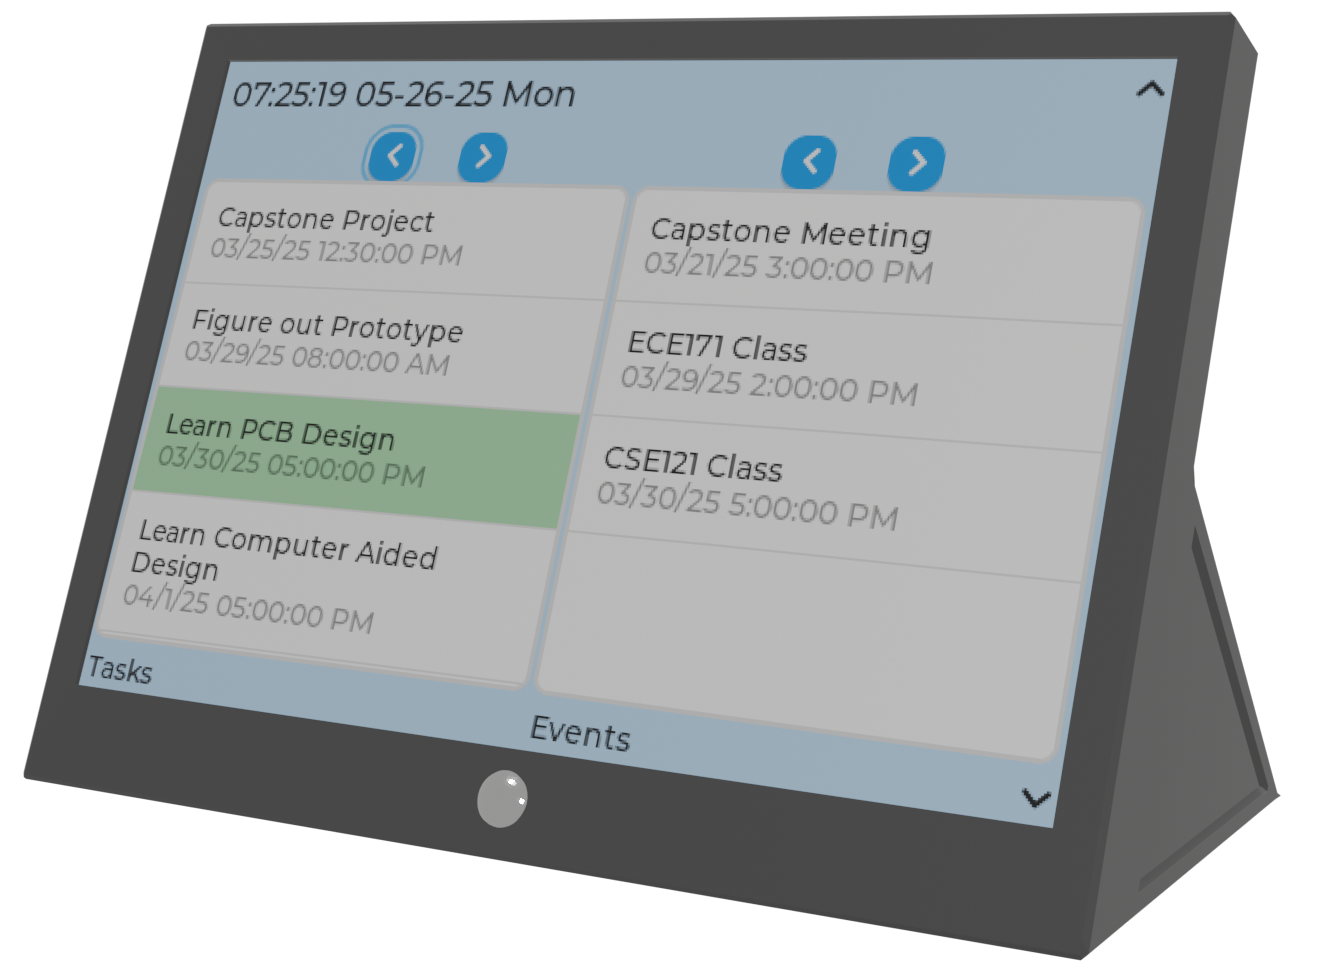
\includegraphics[width=\textwidth]{schedule_companion_render.png}
  \end{minipage}%

  \note[item]{The intent of this project is to facilitate \textit{Goal Completion}, which our task managed through \textit{entry management}}
  \note[item]{Tasks are defined objectives that must be completed by a given deadline.}
  \note[item]{Events represent fixed intervals of time and are recorded within the device’s internal calendar.}
  \note[item]{Habits, in contrast to tasks, represent repeated behaviors the user wishes to cultivate.}
\end{frame}

\begin{frame}
  \frametitle{Prototyped elements of design}
\centering
\small
\begin{tabular}{|p{0.2\textwidth}|p{0.2\textwidth}|p{0.2\textwidth}|p{0.2\textwidth}|}
\hline
\cellcolor[HTML]{CFE2F3}Interactive UI        & Touchscreen                                           & \cellcolor[HTML]{CFE2F3}Web app functionality & \cellcolor[HTML]{CFE2F3}Cloud server functionality \\ \hline
\cellcolor[HTML]{CFE2F3}User account creation & \cellcolor[HTML]{CFE2F3}Wifi Provisioning             & Battery powered                               & \cellcolor[HTML]{CFE2F3}New user creation          \\ \hline
\cellcolor[HTML]{CFE2F3}New device addition                           & \cellcolor[HTML]{CFE2F3}Many devices to one user      & \cellcolor[HTML]{CFE2F3}Offline Usage         & \cellcolor[HTML]{CFE2F3}Real Time Clock display    \\ \hline
\cellcolor[HTML]{CFE2F3}Focus Mode            & \cellcolor[HTML]{CFE2F3}Task and Event Implementation & \cellcolor[HTML]{CFE2F3}Habit Implementation  & Time Blocking                                      \\ \hline
Configurable User Settings                    & End to End encryption                                 & Phone App                                     & Haptics and Audio feedback                         \\ \hline
One device to many users                      & Schedule sorting                                      & Power button                                  &                                                    \\ \hline
\end{tabular}
\end{frame}

\begin{frame}
  \frametitle{Biggest Roadblock: Memory usage}

  The prototype design ran into memory availability issues
  \begin{itemize}
    \item 188 kB of static memory (58.4\% of available memory)
    \begin{itemize}
      \item 66 kB used by graphics
      \item 60 kB used by networking
      \item 133 kB left for dynamic memory
    \end{itemize}
    \item Different features
    \begin{itemize}
      \item BLE for Wifi info
      \item Persistent connection
    \end{itemize}
  \end{itemize}
  ESP32C3 chip is insufficient for the manufactured product.

  \note[item]{GPU option: If we utilized dual cpus for the graphical display, display would be faster}
  \note[item]{LVGL already custom external gpu rendering}
  \note[item]{With more memory and parallel processing, current approach should
  be more performant}
  \note[item]{This taught us our hardware requirements for the manufactured product}

\end{frame}

\begin{frame}
  \frametitle{Wi-Fi and MQTT}

  \begin{itemize}
    \item Wi-Fi provisioning + connection + MQTT = 100 kB (static \& dynamic)
    \item No memory = no persistent session = no stored messages
    \item User makes change $\rightarrow$ need to send entire backup
  \end{itemize}

  An HTTP server that responds to "changes since X" is a more efficient approach.

  \note[item]{persistent sessions store non-ack'd qos = 1 messages}
  \note[item]{after a reconnect, non-ack'd items are re-sent}
  \note[item]{instead of connecting and having a worker thread, the prototype
  connects, spends 5s, then disconnects, ending the session}
  \note[item]{Final product asks for the entire thing on power-on, then react to any
  new messages during the persistent connection.}
\end{frame}
\begin{frame}
    
  \frametitle{What did we learn from the prototype?}

  \begin{columns}
    \column{0.5\textwidth}
    What worked:
    \begin{itemize}
      \item SQLite3
      \item Persistence
      \item Web server
      \item SoftAP Wi-Fi provisioning
    \end{itemize}

    \column{0.5\textwidth}
    What is improved and included in the manufactured product:
    \begin{itemize}
      \item MQTT
      \item Memory usage
      \item SoC specs
      \item Device authentication
      \item End to End Encryption 
      \item Additional software features
      \item Screen size and touch
      \item Haptics and audio 
      \item Bluetooth Wi-Fi provisioning
    \end{itemize}
  \end{columns}

  \note[item]{MQTT: no persistent connection --- no message \textit{queue}}
  \note[item]{ESP32-C3: RISC-V SoCs do not support memory expansion}
  \note[item]{Discuss potential alternatives: ESP32-S3, Teensy 4.1, STM32H7 line, Pi Zero 2W}
  \note[item]{Components: add haptics, audio, improve screen and touch}
  \note[item]{Additional features: time blocks, custom schedule organization}
  \note[item]{Although we can use SoftAP, Bluetooth Wifi provisioning using a phone app is a better user experience}

\end{frame}

\begin{frame}
  \frametitle{Server Architecture}

  \begin{center}
    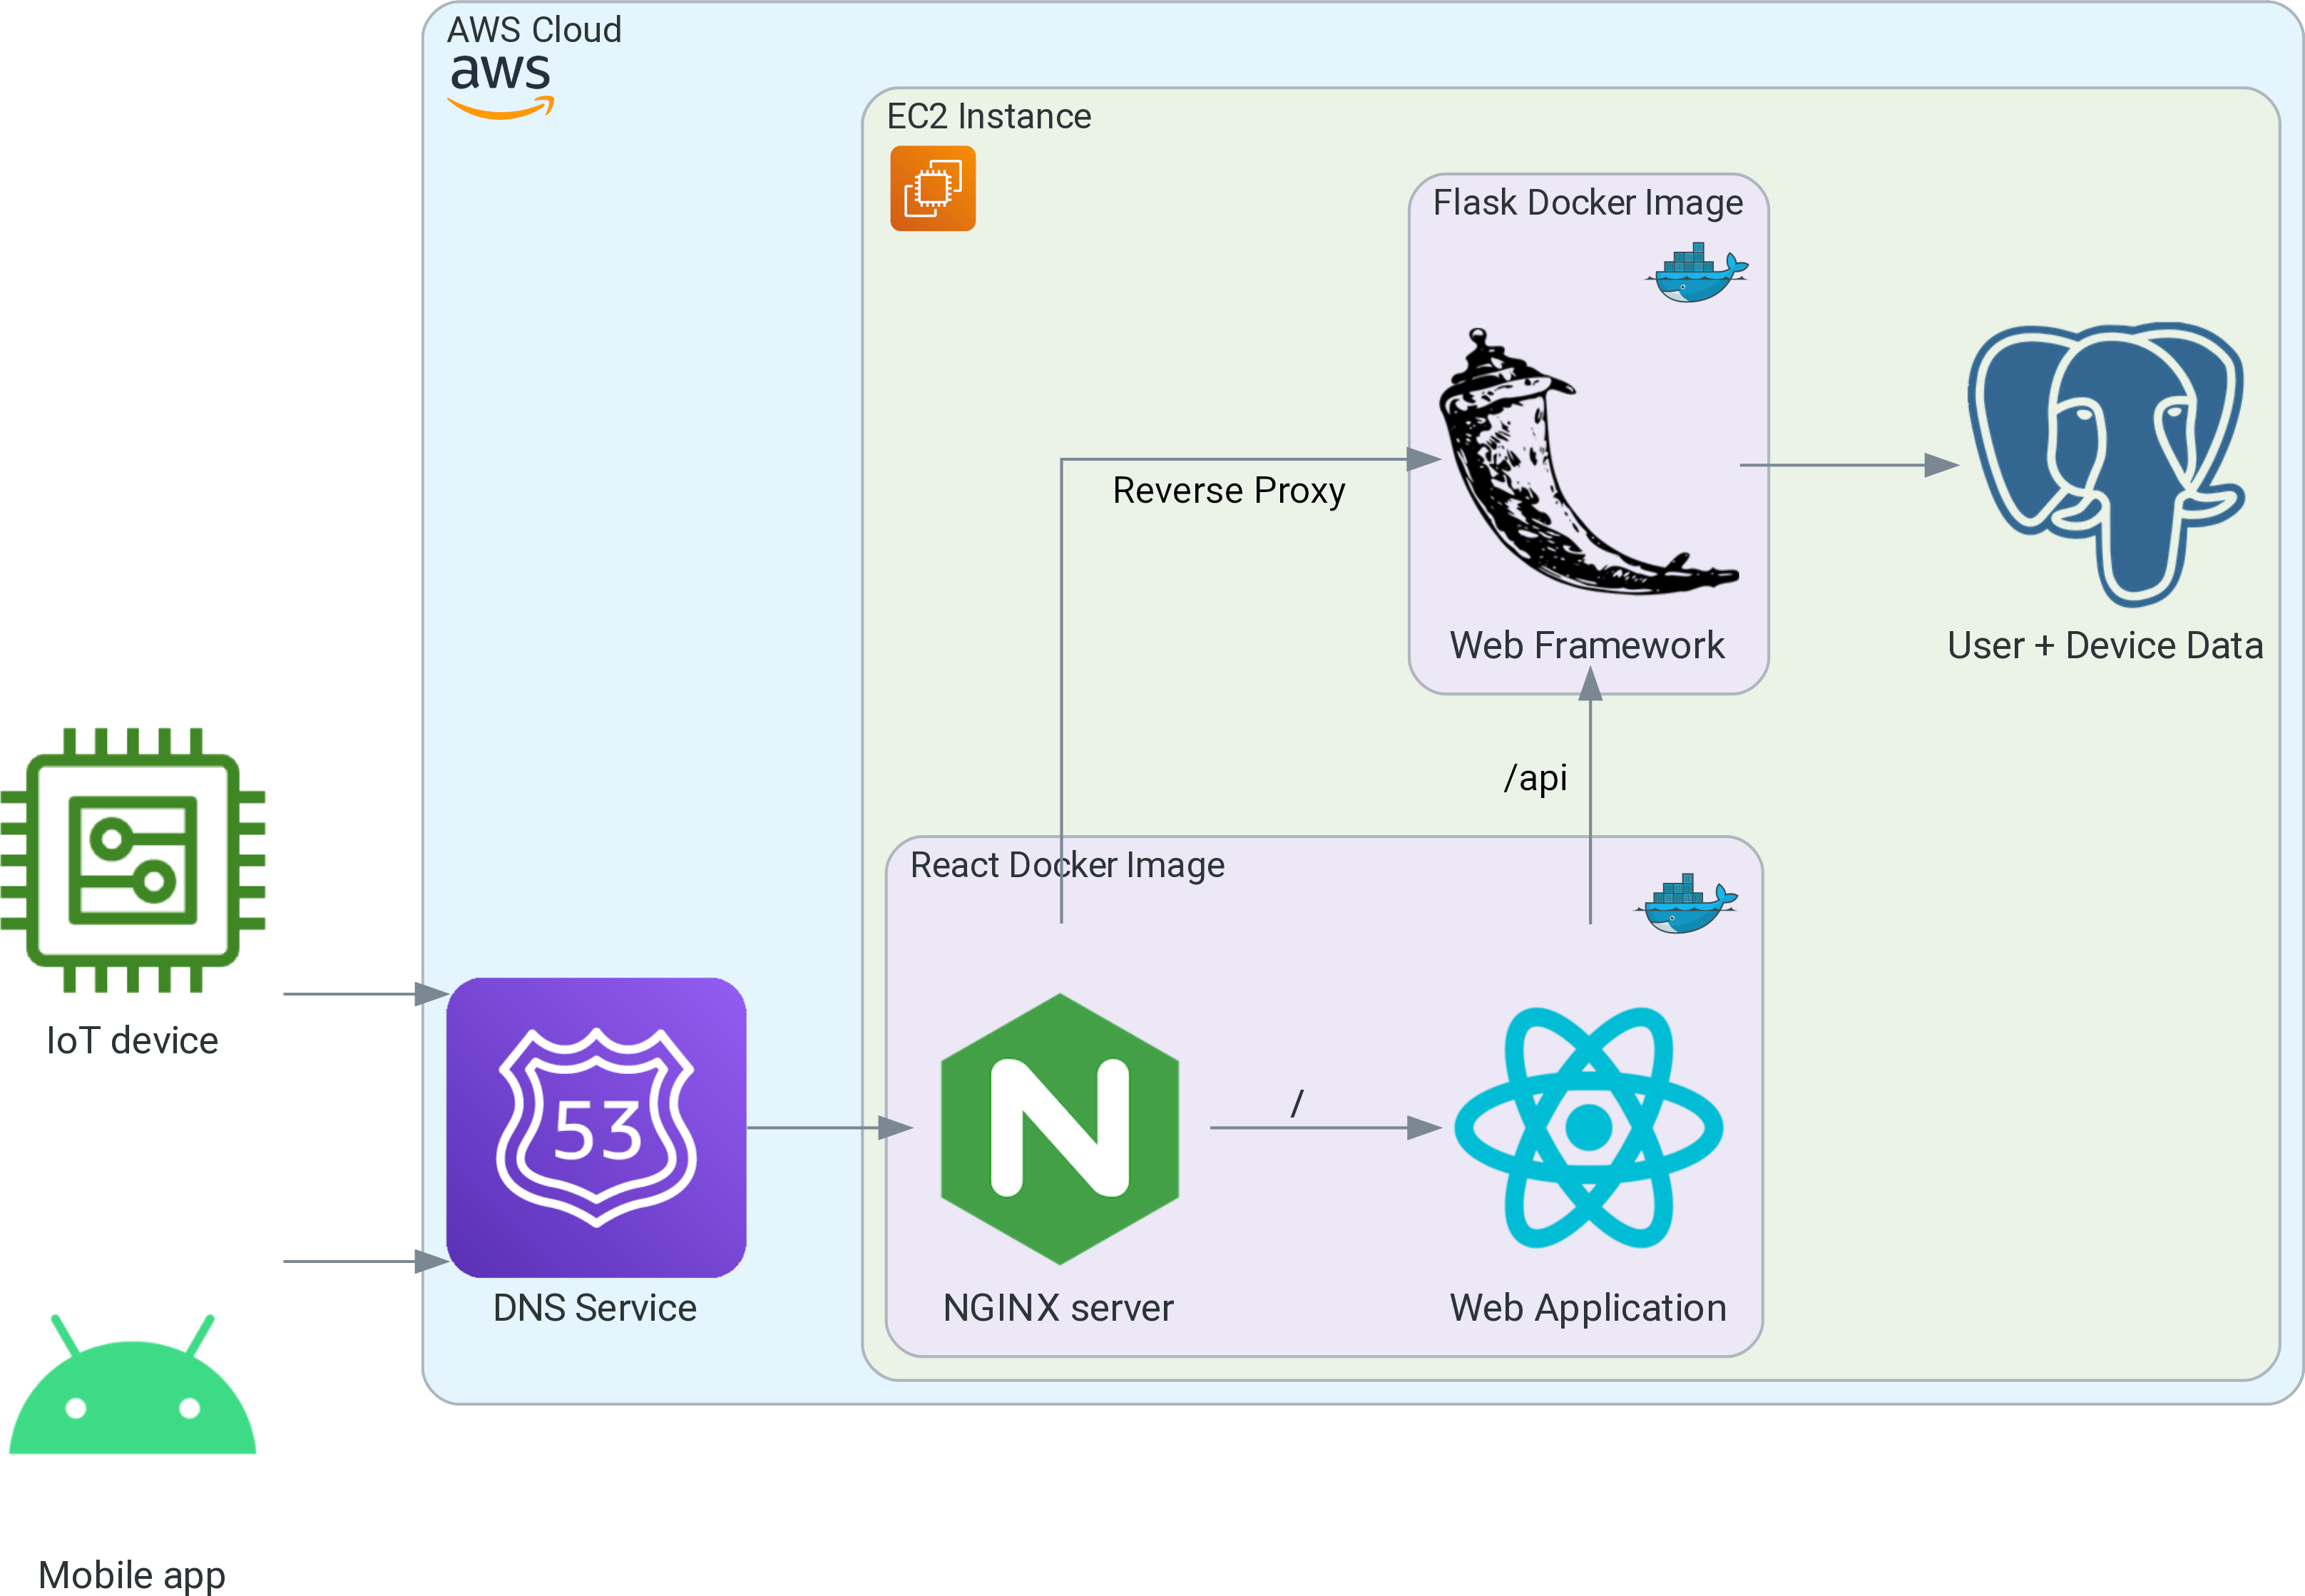
\includegraphics[width = 0.9 \textwidth]{data_flow.png}
  \end{center}

  \note[item]{React web app and the device will make requests to "/api" to
  interact with the server data}
  \note[item]{Both user and device will interact with the api after ensuring
  they have an un-expired jwt}
  \note[item]{With device jwt, we will have better security and a proper
  device authentication process}

\end{frame}

\begin{frame}
  \frametitle{Tests}
  \begin{columns}
    \column{0.5\textwidth}
    Prototype feasible tests:
    \begin{itemize}
      \item Wifi Provisioning
      \item Boot time 
      \item Sync time 
      \item New User Registration 
      \item New Device Addition
      \item Many to One Support 
      \item Data Persistence
    \end{itemize}

    \column{0.5\textwidth}
    Manufactured product tests:
    \begin{itemize}
      \item Durability
      \item Thermal
      \item Battery life cycle
      \item Haptics and sound
    \end{itemize}
  \end{columns}
  \note[item]{Durability testing: includes chemical testing, drop testing, tensile testing, UV testing}
  \note[item]{Battery life cycle: charge speed, battery degradation, battery life}
\end{frame}

\begin{frame}
  \frametitle{Test Results}
    \centering
    \begin{tabular}{l
    >{\columncolor[HTML]{9AFF99}}l }
    \hline
    Test                  & \cellcolor[HTML]{FFFFFF}Results                      \\
    \hline
    Wifi Provisioning     & PASS                         \\
    Boot time             & PASS                         \\
    Sync time             & \cellcolor[HTML]{FFCCC9}FAIL \\
    New User Registration & PASS                         \\
    New Device Addition   & PASS                         \\
    Many to One Support   & PASS                         \\
    Data Persistence      & PASS                         \\
    \hline
    \end{tabular}
\end{frame}

\begin{frame}
  \frametitle{Initial goal}

  \input{build/design_objective_table_md}

  \begin{center}
    Did we succeed?
  \end{center}

  \note[item]{No to sync time}
  \note[item]{Battery seems feasible}
\end{frame}

\begin{frame}
  \frametitle{Finalized Specs}
  \centering
    \begin{tabular}{lllll}
    \hline
    Specifications                & Units   & \multicolumn{3}{l}{Value}                        \\
    \hline
    Price                         & USD     & \textbf{\$100}     & \textbf{$\rightarrow$} & \textbf{\$150} \\
    Devices per user              & Units   & \textbf{Unlimited} & \textbf{$\rightarrow$} & \textbf{10}    \\
    Users per device              & Units   & \textbf{Unlimited} & \textbf{$\rightarrow$} & \textbf{8}     \\
    Cloud sync time               & Seconds & \textbf{10}        & \textbf{$\rightarrow$} & \textbf{5}     \\
    Simultaneous tasks             & Tasks   & \multicolumn{3}{l}{Up to 100}                    \\
    Database Size                 & Bytes   & \multicolumn{3}{l}{60 GB, non-volatile}          \\
    \textbf{Standby} Battery life & Hours   & \textbf{200}       & \textbf{$\rightarrow$} & \textbf{30}    \\
    Wakeup time                   & Seconds & \textbf{3}         & \textbf{$\rightarrow$} & \textbf{2}    \\
    \hline
    \end{tabular}
\end{frame}

\begin{frame}
  \frametitle{Scheduled Activity Design}

  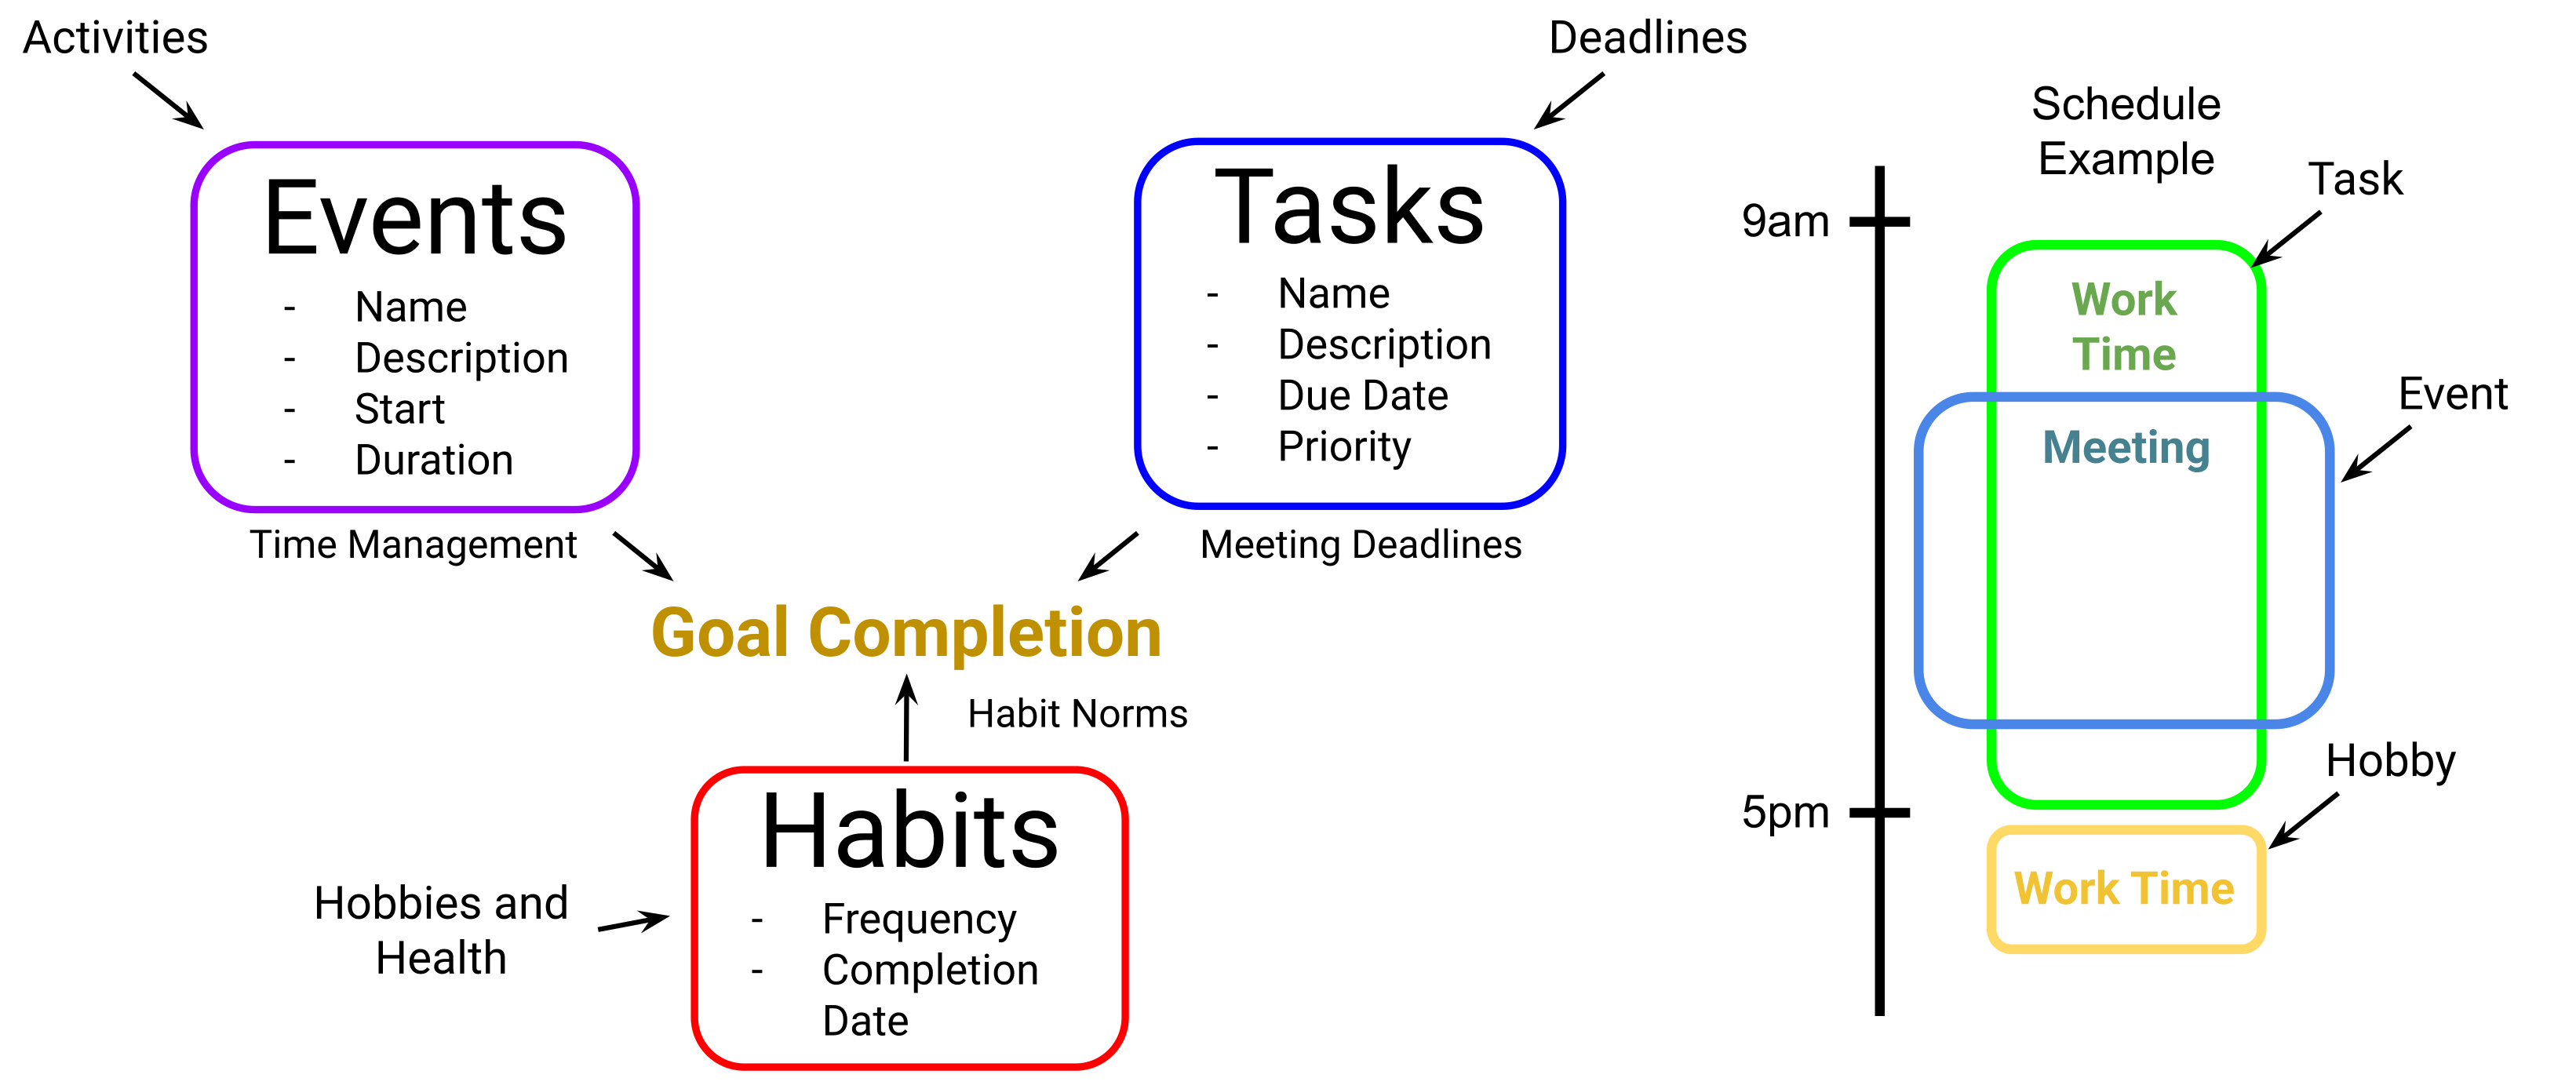
\includegraphics[width=\textwidth]{goal_completion.png}

  
  \note[item]{The triangular volume on the back of the device serves as a kickstand and case for electronics.}
  \note[item]{Keeps center of gravity low makes it difficult to tip over}
  \note[item]{A large space is necessary to fit two 18650 battery cells which we selected over a specific pouch battery for repairability}
  \note[item]{Provides room for easily assembly and disassembly, good for repairability.}

\end{frame}


\end{document}
